\documentclass[letterpaper]{article}
\usepackage{aaai23}
\usepackage{times}
\usepackage{helvet}
\usepackage{courier}
\usepackage[hyphens]{url}
\usepackage{graphicx}
\urlstyle{rm} 
\def\UrlFont{\rm}  
\usepackage{natbib}
\usepackage{caption}
\usepackage{tikz}
\frenchspacing  
\setlength{\pdfpagewidth}{8.5in}  
\setlength{\pdfpageheight}{11in}  

\title{Crafting the Ultimate Digital Dungeon Master Using GPT Models}
\author{Robert Nasuti\\
University of Colorado at Colorado Springs\\
rnasuti@uccs.edu}

\begin{document}

\maketitle

\begin{abstract}
    This paper delves deeper into the pioneering approach of harnessing a state-of-the-art Large Language Model (LLM), specifically GPT-4, to act as a dynamic and interactive dungeon master for digital role-playing games. Building upon an initial proposal, we detail the development and refinement of a custom framework tailored to complement the LLM's narrative capabilities. This endeavor not only enriches digital gaming experiences but also underlines the expansive possibilities of LLMs in sculpting adaptive and responsive AI-driven systems. With advancements in memory management, user interface design, and evaluation techniques, we present a comprehensive overview of our journey in redefining digital role-playing, distinguishing our approach through its unique integration of AI and gaming.
\end{abstract}

\section{Introduction}
The allure of digital role-playing games (RPGs) has consistently stemmed from their promise of immersive universes, rich narratives, and the freedom for players to forge their own paths. The linchpin of many such experiences, especially in tabletop RPGs like Dungeons \& Dragons, is the dungeon master (DM) – an entity that meticulously crafts the narrative tapestry, molding it in real-time based on players' choices. While the role of a DM has traditionally been occupied by humans, the meteoric rise in the capabilities of Large Language Models (LLMs) prompts a fascinating question: Can we recreate the dynamism, creativity, and adaptability of a human DM using state-of-the-art AI?

Our prior work proposed the potential of LLMs in this realm, drawing parallels with their success in mimicking complex human behaviors and interactions. As we progress further into our research, this paper presents a detailed exploration of the strides made in realizing this vision. From building a robust framework that synergizes with the LLM's strengths to grappling with challenges in memory, user interface, and function calling, we offer a deep dive into the intricacies of crafting the ultimate digital DM. As the boundaries between human creativity and machine-generated content blur, our work stands at the forefront of this intersection, seeking to redefine interactive gaming experiences for the digital age.

\section{Project Context and Recap}
At the heart of this project lies the challenge of transforming the traditional role of a dungeon master (DM) in role-playing games into a digital, AI-driven counterpart. The goal has been to develop a Digital DM that offers:
\begin{itemize}
\item An intuitive User Interface,
\item Effective Game State Maintenance,
\item Comprehensive Game Knowledge,
\item Efficient Character and Story Management, and
\item A Dynamic Interactive Dialog System.
\end{itemize}
With these foundational requirements in mind, our journey has been centered around crafting a system that seamlessly integrates these elements while leveraging the unparalleled capabilities of Large Language Models. In the sections that follow, we delve into the specific frameworks and tools employed, the challenges encountered, and the solutions devised in our endeavor.

\section{Custom Framework}

\subsection{Backend}

\subsubsection{Memory Management}
The core of the Digital DM's backend is its memory management system. This system is bifurcated into:

\paragraph{Short-Term Memory:}
Large Language Models (LLMs) like GPT fundamentally operate as stateless sequence-to-sequence models. This characterization is crucial to understanding their short-term memory capabilities. Specifically, their short-term memory is encapsulated in the conversation history, which forms the basis of their input sequence, commonly referred to as the "prompt." The model processes this prompt and generates a response, known as the "completion," forming the output sequence. Crucially, the combined length of the prompt and completion must not exceed the model's maximum context window. This limitation necessitates efficient management of this limited context window to maintain narrative continuity and coherence in complex scenarios.

Our custom implementation addresses these constraints through the \textit{Conversation} class\footnote{Available at: \url{https://github.com/rlnasuti/DungeonMasterBot/blob/main/bot/models/conversation.py}}. This class is specifically designed to handle the dynamic summarization and manage the token constraints of the LLM, ensuring the conversation remains within the model's token limits. Key features include:

\begin{itemize}
\item \textbf{Dynamic Token Counting}: Utilizing the tiktoken library, the system dynamically tracks the token count, keeping the conversation within the model's token constraints.

\item \textbf{Message Roles in the Digital DM Framework}: 
Different message roles within the conversation history are managed meticulously:
\begin{itemize}
    \item \textit{System Messages}: Set the assistant's behavior or tone at the conversation's outset. Absent such a message, the system defaults to general helpful behavior.
    
    \item \textit{User Messages}: Inputs from players, crucial for contextualizing the assistant's coherent responses.
    
    \item \textit{Assistant Messages}: The assistant's responses, vital for dialogue continuity. Predefined messages can exemplify desired behavior.
    
    \item \textit{Function Messages}: Enable invoking specific functions from the OpenAI API, informing the model of function outcomes for future interactions.
\end{itemize}

\item \textbf{Adaptive Summarization}: Activated when a new message risks exceeding the token limit. Older messages are condensed into succinct summaries, replacing detailed history to conserve tokens while retaining narrative continuity. These summaries are also logged for reference. This approach is in line with the methods suggested by Wang et al. \cite{wang2023recursively}, who propose recursively generating summaries using LLMs to enhance long-term memory in dialogue systems.

\item \textbf{Detailed Logging}: Every modification or addition to the conversation is cataloged, offering insights into token counts and the conversation's evolution. This record aids both in debugging and understanding the system's decision-making.
\end{itemize}

\paragraph{Long-Term Memory:}
To address the limitations of the model's immediate context window, our system employs a sophisticated long-term memory mechanism using embeddings. Embeddings from a rich corpus of sourcebooks, rulebooks, and prior interactions are created using OpenAI's text-embedding-ada-002 model and stored in a vector database named `Weaviate`.

The retrieval of information from this vector database is seamlessly integrated into the model's workflow through a process known as "Retrieval Augmented Generation" (RAG). In this process, when the model requires additional information, it issues a function call that triggers the following steps:
\begin{enumerate}
    \item The query or question from the model is transformed into an embedding.
    \item This embedding is used to search the vector database for similar embeddings, effectively querying the long-term memory.
    \item The most relevant retrieval from the vector database is then injected into the model's prompt as additional context.
\end{enumerate}
This approach ensures that the model has access to a broader range of information beyond its immediate context window, enhancing the richness and accuracy of its responses. By leveraging the RAG pattern, the system effectively bridges the gap between the model's short-term memory limitations and the expansive universe of the game narrative, ensuring continuity and depth in the Digital DM's storytelling.


\subsubsection{Agentic Framework}
The Agentic Framework is the heart of the Digital DM, driving the narrative and managing game dynamics. It's designed to handle user interactions and ensure that the system responds adaptively, maintaining the dynamism inherent to RPGs.

This framework is built using Python and utilizes the OpenAI API for generating responses. It processes user messages, adds them to the conversation history, and creates a prompt for the AI model. The system then iteratively communicates with the model, handling any function calls and incorporating the responses into the ongoing conversation. This iterative process allows the Digital DM to adapt its responses based on the evolving game context, ensuring a responsive and dynamic narrative flow.

A visual representation of this control loop is depicted in Figure \ref{fig:control_loop}.

\begin{figure}[h]
    \centering
    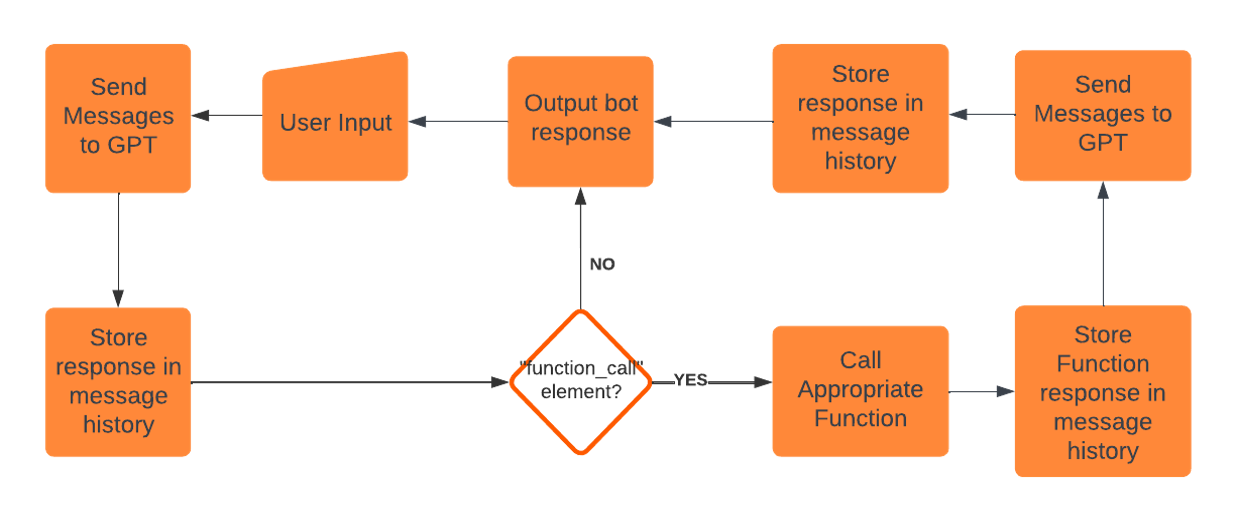
\includegraphics[width=\linewidth]{control_loop.png}
    \caption{The Agentic Framework Control Loop.}
    \label{fig:control_loop}
\end{figure}

\subsection{Frontend}
\subsubsection{User Interface (UI)}
For the frontend, the project utilizes \texttt{Chainlit}, an open-source Python package, chosen for its exceptional suitability in creating a responsive and intuitive UI for the Digital DM. The UI is designed to facilitate smooth player interactions with the system.

The UI is designed to facilitate smooth player interactions with the system. It handles the streaming of messages, both from the user and the AI, and manages the display of function call responses. The UI also plays a crucial role in maintaining the conversation's flow, ensuring that players have a seamless gaming experience.

The Chat completions API\footnote{For more information, see: \url{https://platform.openai.com/docs/guides/gpt/chat-completions-api}} is structured to facilitate multi-turn conversations using a list of messages. Each message has a designated role, which can be one of three types: "system", "user", or "assistant". The sequence and roles of these messages are pivotal in guiding the behavior of the LLM and in directing the conversation.

\subsubsection{Context Management}
To ensure a logical flow in the conversation, it's crucial to maintain a history of prior messages. The assistant lacks inherent memory of past requests; thus, relevant information must be supplied within the conversation history. If a conversation exceeds the model’s token limit, the API will return an error.

\subsubsection{Function Calling in the Chat completions API}
The latest models in the Chat completions API are designed to describe and call functions, generating a JSON object containing arguments for those functions. This feature enables more structured and dynamic interactions with the assistant.

\subsubsection{Function Integration}
Functions are embedded into the system message in a syntax familiar to the model. These functions are then counted against the model's context limit and are billed as input tokens. This approach ensures that the assistant can interpret and utilize the functions as intended.

\subsubsection{Application Scenarios}
Function calling offers several applications:
\begin{itemize}
    \item Constructing chatbots that invoke external APIs.
    \item Transforming natural language queries into specific API calls.
    \item Extracting structured data from text.
\end{itemize}

\subsubsection{Function Calling Procedure}
The procedure involves:
\begin{enumerate}
    \item Making an initial call to the model with the user's query and a set of functions.
    \item The model chooses to call a function, producing a stringified JSON object.
    \item Parsing the JSON in your code and invoking your function using the provided arguments.
    \item Making a subsequent call to the model, incorporating the function response, allowing the model to summarize the results to the user.
\end{enumerate}

\subsubsection{Note on Function Calling}
While function calling adds versatility to the assistant, it also introduces potential risks. It's crucial to incorporate user confirmation flows before performing impactful real-world actions, such as sending emails or making online posts, to ensure user intent is accurately captured and acted upon.

\section{Evaluation}

The evaluation of our Digital DM is conducted through two primary methodologies: the qualitative "Vibe Check" and the more structured "LLM-as-a-Judge" approach.

\subsection{Vibe Check}
The "Vibe Check" method serves as our initial evaluation stage. Analogous to unit testing in traditional software development, this process involves engaging in conversations with the model to ascertain the quality of its responses. The focus is on ensuring that the model's replies not only align with the context and narrative of the game but also possess the creativity and dynamism expected from a human DM.

During this stage, various scenarios and dialogues are spot-checked. The purpose is to intuitively assess the model's performance, gauging its ability to handle unexpected player inputs, maintain narrative coherence, and add depth to the game's storyline. While this method provides valuable immediate feedback, it's inherently subjective and doesn't scale well for comprehensive testing. It serves as a preliminary check before more systematic evaluation methods are applied.

\subsection{LLM-as-a-Judge}
To supplement the qualitative insights from the "Vibe Check," we introduce the "LLM-as-a-Judge" method \cite{zheng2023judging} for a more structured evaluation. This approach involves codifying test cases in the form of prompts, which include message histories, and defining ideal completions for these prompts. The test cases are then run through the system, with the generated responses being saved for evaluation.

The core of the "LLM-as-a-Judge" method is in its grading system. The saved responses, along with the ideal completions, are presented to an independent LLM. This LLM acts as a judge, evaluating and grading the responses against the ideal completions. The grading is done on a scale, such as 1-5 or traditional academic grades (A, B, C, D, F). To guide the grading LLM, examples of what constitutes each rank or grade are provided, ensuring a consistent evaluation metric.

This method allows for a more objective assessment of the Digital DM's performance, quantifying its ability to handle predefined scenarios and comparing its outputs to an ideal standard. By incorporating both the "Vibe Check" and "LLM-as-a-Judge" methods, we aim to capture both the subjective experience of interacting with the Digital DM and an objective measure of its capabilities.

\section{Next Steps}
Moving forward, our project aims to enhance the user interface, improve the bot's capabilities, refine the user experience, and establish a rigorous testing framework. These improvements are outlined in detail below:

\subsection{UI Enhancement}
\textbf{Add "Roll Dice" Button:} Introduce an interactive feature allowing users to simulate dice rolls within the UI, thereby enriching the game experience and facilitating decision-making processes integral to gameplay.

\subsection{Bot Enhancements}
\begin{itemize}
\item \textbf{Memory Fragments:} To enhance continuity and context-awareness, the bot will store past interactions in a vector format. During each user interaction, it will retrieve a set number of these fragments, ensuring a more coherent and personalized interaction history.
\item \textbf{Narrative Anchors:} By leveraging chapter summaries and pivotal plot points, combined with the aforementioned "Memory Fragments," the bot will anchor its responses and storytelling to key narrative elements. This integration will foster more consistent and engaging storytelling.
\item \textbf{Character Cards:} To further enrich the role-playing aspect, we plan to introduce "Character Cards" that serve as system prompts for GPT. These cards will be activated when GPT assumes in-game character roles, providing a structured framework for character-driven narratives.
\end{itemize}

\subsection{User Experience}
\begin{itemize}
\item \textbf{Refactor "Character Creation" to a Dedicated Screen:} To streamline the character creation process and enhance user engagement, we will develop a dedicated interface specifically for character customization and creation.
\item \textbf{Stretch Goal - Integrate DallE-3 for Character Portrait Generation:} As an ambitious goal, we aim to incorporate DallE-3 technology to generate unique and personalized character portraits, adding a visual dimension to the user's imaginative experience.
\end{itemize}

\subsection{Testing}
\begin{itemize}
\item \textbf{Develop a Comprehensive Evaluation Set:} To ensure the robustness and reliability of our enhancements, we will compile a comprehensive set of evaluation criteria and test cases.
\item \textbf{Establish a Robust Testing Framework:} Building a structured and systematic testing framework will be crucial for assessing the functionality and effectiveness of the proposed enhancements. This framework will enable us to identify and address potential issues proactively.
\end{itemize}

These steps are designed to propel the project forward, addressing critical areas of improvement to deliver a more immersive, coherent, and engaging user experience.

\section{Conclusion}
As we reach the midpoint of this ambitious project, it is clear that the journey to craft the ultimate Digital Dungeon Master using GPT models is well underway. The progress made thus far is significant, laying a solid foundation for the transformative potential of Large Language Models in digital role-playing games. Our custom framework, designed to synergize with the LLM's narrative capabilities, has begun to take shape, showing promising results in memory management, user interaction, and dynamic storytelling.

While the journey is far from complete, the strides made thus far are encouraging. The backend and frontend frameworks, the Agentic Framework, and the initial evaluation strategies have all been successfully implemented, providing a glimpse into the transformative potential of this endeavor. The challenges encountered have been valuable learning opportunities, helping refine our approach and methodology.

Looking ahead, there is much to be done. The next phase of the project will focus on enhancing the user interface, further improving the bot's capabilities, refining the user experience, and establishing a rigorous testing framework. These enhancements are crucial in realizing the full potential of the Digital DM, ensuring a seamless and immersive gaming experience.

As we continue on this exciting journey, the goal remains clear: to redefine digital role-playing by creating an AI-driven Dungeon Master that rivals the creativity, adaptability, and dynamism of a human counterpart. The progress made thus far is a testament to the potential of this endeavor, and the remainder of this semester promises to be a period of significant advancement and innovation.

\section*{Acknowledgments}
I'd like to thank ChatGPT \cite{ChatGPT2023} for assistance with formatting, editing, and LaTeX support throughout this assignment.

\bibliography{aaai23}

\end{document}

